\section{Calibration and Amplification Fail}
\label{sec:calib}

The grid says that trigger-aware repair is the only family that tolerates
imperfect recall, and that it needs the trigger. Two natural responses are to
avoid the trigger requirement through calibration and to rescue deletion by
making the poison it missed easier to find. We tried both. Neither works under
our pre-registered criteria.

\subsection{Calibrate-then-Remove}
CaR uses a synthesised trigger as a proxy for the real one. For each
spectral-signature threshold $\theta$, it builds the corresponding forget set,
runs the recipe's repair stage, and measures the proxy-removed model's response
$\tau$ to the synthesised pattern. A threshold is acceptable only if
$\tau\leq5\%$, because a model that no longer responds to the proxy is presumed
not to respond to the real trigger either. If no threshold qualifies, the method
falls back to the F1-optimal one.

Table~\ref{tab:car} reports the sweep. Across twenty thresholds, $\tau$ is
100\% in nineteen cases and 97.5\% in the remaining one. The proxy pattern is
optimised on the poisoned model and has zero intersection with the true patch, so
label repair does not remove the model's response to it; the calibration signal
is saturated regardless of how much poison the threshold captures. The recall of
the sweep ranges from 0.003 to 1.000 and its precision from 0.333 to 1.000, so
the sweep does cover the useful range. The best F1 is 0.918 at recall 0.894 and
precision 0.942, and the model produced there still has ASR $99.97\%$ and clean
accuracy $86.71\%$. The CaR rule never fires, the fallback is taken, and the
fallback does not remove the backdoor.

The failure is instructive. A calibration guarantee is only as good as the
exchangeability between the calibration signal and the test signal. Here the
proxy is a different pattern, optimised for a different purpose, and the repair
stage is not designed to suppress it. The guarantee is vacuous before any
threshold is chosen.

\begin{table}[t]
\centering
\caption{E3: Calibrate-then-Remove fails because the proxy signal is uninformative.}
\label{tab:car}
\footnotesize
\begin{tabular}{ccccccc}
\toprule
\textbf{$\theta$} & \textbf{Recall} & \textbf{Precision} & \textbf{$\tau$} & \textbf{F1} & \textbf{Clean} & \textbf{ASR} \\
\midrule
0.01 & 1.000 & 0.333 & 97.5 & 0.500 & 82.32 & 99.78 \\
20.71 & 1.000 & 0.396 & 100.0 & 0.567 & 88.01 & 100.00 \\
35.33 & 0.998 & 0.486 & 100.0 & 0.654 & 88.77 & 100.00 \\
50.23 & 0.992 & 0.628 & 100.0 & 0.769 & 88.88 & 100.00 \\
74.23 & 0.956 & 0.863 & 100.0 & 0.907 & 89.19 & 100.00 \\
127.71 & 0.633 & 0.999 & 100.0 & 0.775 & 89.20 & 100.00 \\
191.72 & 0.161 & 1.000 & 100.0 & 0.277 & 89.29 & 99.98 \\
291.83 & 0.003 & 1.000 & 100.0 & 0.006 & 89.22 & 99.98 \\
\midrule
F1-optimal & 0.894 & 0.942 & 100.0 & 0.918 & 86.71 & 99.97 \\
\bottomrule
\end{tabular}
\par\vspace{1pt}\footnotesize\raggedright Calibrate-then-Remove, seed 0. $\theta$ is the Spectral-Signature threshold, $\tau$ the trigger response of the proxy-removed model (\%). Nineteen of twenty thresholds give $\tau{=}100\%$ and the twentieth $97.5\%$: the synthesised trigger never elicits the backdoor (IoU $=0.000$ against the true patch), so no threshold satisfies $\tau\leq5\%$ and CaR degenerates to its fallback. Both the F1-optimal and the CaR choice leave ASR $\approx100\%$.
\end{table}


\subsection{The Ascent Artefact}
A second attempted rescue is to forget harder. Feature-space ascent on the forget
set is a standard unlearning baseline, and in our first runs it appeared to work:
at learning rate $10^{-3}$ for two epochs, ASR fell to $0.18\%$ and at four
epochs to $0.00\%$ (Table~\ref{tab:e8}, Fig.~\ref{fig:ascent}). Clean accuracy
fell with it, to $85.29\%$ and then to $77.25\%$, which we initially read as the
usual utility cost of unlearning.

The reading was wrong. Batch normalisation maintains running estimates of
activation statistics, and ascent updates them along with the weights. Re-running
the identical schedules with the batch-norm statistics frozen to those estimated
on the retained set removes the apparent effect entirely: ASR is
$99.94$--$99.98\%$ at every learning rate, with clean accuracy $88.72$--$88.74\%$
and no utility loss at all. The backdoor was never removed; the normalisation
layers were corrupted, and the corrupted statistics made the trigger inoperative
while also damaging clean accuracy. A reader who evaluates unlearning without a
normalisation control can therefore report a successful removal that is an
artefact of the evaluation pipeline.

Label repair at comparable strength behaves differently. At learning rate
$0.005$ for two epochs ASR is $10.11\%$ with clean accuracy $87.91\%$; at $0.01$
for one epoch it is $16.36\%$ with $87.15\%$; a re-run of the same cells gave
$8.63\%$ and $15.11\%$. These are genuine reductions, achieved without damaging
the network, but they are above the 5\% threshold. Repair needs the inoculation
stage to cross it.

\begin{table}[t]
\centering
\caption{E8: ascent-based 'removal' is a normalisation artefact.}
\label{tab:e8}
\footnotesize
\begin{tabular}{llcc}
\toprule
\textbf{Variant} & \textbf{Setting} & \textbf{Clean} & \textbf{ASR} \\
\midrule
Raw ascent & lr0.0002 ep2 & 88.03 & 18.06 \\
Raw ascent & lr0.0005 ep2 & 87.31 & 2.87 \\
Raw ascent & lr0.001 ep2 & 85.29 & 0.18 \\
Raw ascent & lr0.001 ep4 & 77.25 & 0.00 \\
BN-guarded ascent & lr0.0002 ep2 & 88.74 & 99.98 \\
BN-guarded ascent & lr0.0005 ep2 & 88.72 & 99.98 \\
BN-guarded ascent & lr0.001 ep2 & 88.72 & 99.97 \\
BN-guarded ascent & lr0.001 ep4 & 88.73 & 99.94 \\
Label repair & lr0.005 ep2 & 87.91 & 10.11 \\
Label repair & lr0.01 ep1 & 87.15 & 16.36 \\
Label repair (v2) & lr0.005 ep2 & 87.94 & 8.63 \\
Label repair (v2) & lr0.01 ep1 & 87.45 & 15.11 \\
\bottomrule
\end{tabular}
\par\vspace{1pt}\footnotesize\raggedright Seed 1. Raw feature-space ascent appears to remove the backdoor only by destroying the network: clean accuracy falls from $88.03\%$ at the gentlest setting to $77.25\%$ at lr $10^{-3}$ for four epochs, 11.4 points below the gold mean. Re-running the identical schedule with batch-norm statistics frozen to the retain set leaves ASR at $\approx100\%$: the apparent removal was BN corruption, not unlearning. Label repair at the same strength reduces ASR while keeping clean accuracy within 1.5 points.
\end{table}


\begin{figure}[t]
\centering
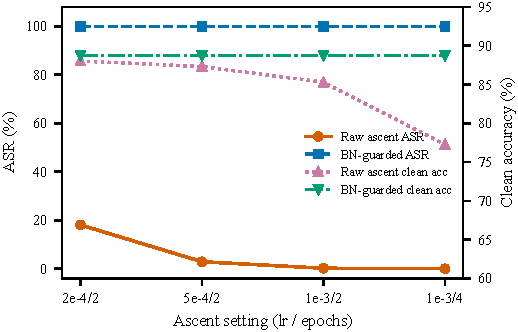
\includegraphics[width=\columnwidth]{fig5_e8_ascent.pdf}
\caption{Raw feature-space ascent appears to remove the backdoor while clean
accuracy collapses; the identical schedules with batch-norm statistics frozen to
the retain set leave ASR at 100\%. The apparent removal is a normalisation
artefact.}
\label{fig:ascent}
\end{figure}

\subsection{The Amplification Hypothesis}
If partial unlearning cannot remove the missed poison, can it at least make that
poison easier to detect afterwards? The hypothesis is plausible: if the network
must support the backdoor on a smaller set of poisoned samples, it may allocate
more capacity to them, and their representations may separate more cleanly from
clean data. If true, the right response to imperfect recall would be an
amplify-and-detect loop: partially remove, re-detect the residue, remove again.

We tested the hypothesis with a pre-registered promotion gate. Partial label
repair was applied at two strengths on the 5\%-poison ResNet-18/BadNets and
ResNet-18/Blend models, and a spectral-signature score was fitted to separate
the missed poison from clean target-class data. The gate required an AUC gain of
at least $+0.10$ over the base model, a clean-accuracy loss of at most two
points, and a gain larger than a matched control that received the same
intervention on clean data instead of poison, on all seeds.

Fig.~\ref{fig:spike} shows the outcome on two seeds. The base models sit at AUC
0.507--0.549 with ASR 99.6--99.8\% and clean accuracy 63.5--63.9\%. Six repaired
models were run. All of them reduce ASR (to between 0.31\% and 87.85\%) and all
raise AUC relative to their base, to between 0.569 and 0.672. But every one of
them also loses clean accuracy: the smallest loss is 2.2 points, and the range is
53.9--61.3\%. The highest AUC, 0.672, occurs at ASR $0.31\%$ and clean accuracy
$55.68\%$; the next, 0.650, at ASR $58.44\%$ and clean accuracy $59.58\%$. The matched
clean-removal controls, which apply the same procedure to clean data instead of
poison, stay at AUC 0.494--0.550 with clean accuracy 62.3--63.3\%. The pattern is
that of a damaged network whose features separate everything a little better, not
of a backdoor made salient: the amplification signal and the utility loss arrive
together. No repaired row remains within two points of its base clean accuracy,
so the pre-registered gate fails on the utility clause even in the rows where the
AUC clause passes.

\begin{figure}[t]
\centering
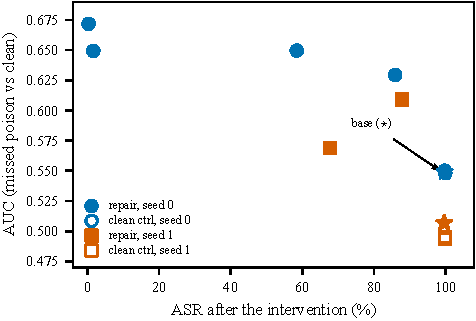
\includegraphics[width=\columnwidth]{fig11_spike_auc.pdf}
\caption{Detectability of missed poison after partial label repair. Filled
markers are repaired models, open markers are matched clean-removal controls,
stars are the poisoned base. AUC rises only where clean accuracy has fallen by
2--10 points; the controls stay at chance.}
\label{fig:spike}
\end{figure}

\subsection{Full-Scale Test}
The spike used 5\% poison and a partial repair. To test the hypothesis at the
scale where it would matter, we repeated it with 10\% poison, three seeds, two
repair strengths, and matched controls (Table~\ref{tab:e9}, Fig.~\ref{fig:amplify}).
The base models have AUC 0.494--0.499. Repair at learning rate $0.005$ gives
0.470--0.497; repair at $0.01$ gives 0.468--0.500. The controls give
0.492--0.503. Every value is at chance, and the largest gain over the base mean
of 0.496 is 0.006. It comes from a control, not from a repaired model; the
largest repair gain is 0.003. Both are two orders of magnitude below the gate of
$+0.10$.

The repair does reduce ASR, from 99.99--100.00\% to 11.07--33.03\%, and it does
so with clean accuracy between 86.81 and 88.20\%, within the two-point budget of
the gold models on every seed. So partial repair is a real
mitigation. What it is not is an amplifier: the poison it fails to remove is no
easier to detect than before. The pre-registered gate fails on its AUC clause on
every seed; it also fails the control clause, because the controls are at chance
and therefore not distinguishable from the repair in the direction the hypothesis
predicts.

\begin{table}[t]
\centering
\caption{E9: the amplification effect does not survive at full scale.}
\label{tab:e9}
\footnotesize
\setlength{\tabcolsep}{5pt}
\begin{tabular}{lccc}
\toprule
\multicolumn{4}{@{}l}{\emph{(a) AUC separating missed poison from clean class-0 data}}\\
\textbf{Condition} & \textbf{Seed 0} & \textbf{Seed 1} & \textbf{Seed 2} \\
\midrule
Base & 0.494 & 0.499 & 0.496 \\
Repair, lr 0.005 & 0.470 & 0.497 & 0.487 \\
Repair, lr 0.01 & 0.468 & 0.476 & 0.499 \\
Clean control, lr 0.005 & 0.492 & 0.499 & 0.501 \\
Clean control, lr 0.01 & 0.495 & 0.503 & 0.501 \\
\midrule
\multicolumn{4}{@{}l}{\emph{(b) Repair outcomes (lr 0.005 / lr 0.01)}}\\
\textbf{Seed} & \textbf{ASR (\%)} & \textbf{Clean acc.\ (\%)} & \\
\midrule
0 & 11.1 / 33.0 & 88.2 / 86.8 & \\
1 & 15.9 / 17.7 & 88.1 / 86.9 & \\
2 & 21.3 / 29.6 & 88.1 / 87.3 & \\
\bottomrule
\end{tabular}
\par\vspace{1pt}\footnotesize\raggedright 10\% poison, simulated recall-0.5 flags. AUC separates the 2{,}500 \emph{missed} poison samples from clean class-0 data. Partial label repair lowers ASR but does not raise AUC above the base model by more than $0.003$ in any seed; the matched clean-removal controls keep ASR at 99.94--100.00\% and clean accuracy at 86.7--87.8\%, and their AUC sits at chance. The pre-registered promotion gate ($\geq+0.10$ AUC, $\leq2$ points clean loss, beating control) fails on every clause.
\end{table}


\begin{figure}[t]
\centering
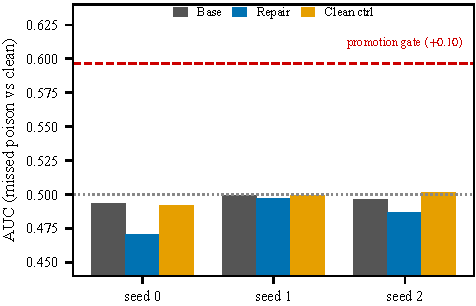
\includegraphics[width=\columnwidth]{fig6_e9_amplify.pdf}
\caption{AUC separating missed poison from clean target-class data at 10\%
poison, three seeds. Partial repair (red) and matched clean-removal controls
(orange) both sit at chance; the dashed line is the pre-registered promotion
gate at base $+0.10$.}
\label{fig:amplify}
\end{figure}

\subsection{What the Failures Have in Common}
Both refinements try to avoid the recipe's dependence on the trigger, and both
fail for the same underlying reason: they need a signal that distinguishes poison
from clean data without knowing what the trigger is. CaR's proxy is a different
pattern and is never suppressed; the amplification hypothesis assumes that the
residual poison becomes more salient, and it does not. The only method in our
suite that crosses the 5\% threshold under imperfect recall is the one that uses
the true trigger. That is a negative result about the state of post-training
removal, and we report it as one.
